\section{Data}
\label{sec:data}

\subsection{Advertising Spending}

I have collected data on government advertising spending (COMSOC), which includes the date (at the daily level) each contract was enforced, the name of the media outlet receiving funds, the name of the government agency contracting the media services or purchasing airtime, and the amount of money allocated. 


Figure \ref{fig:number_of_contracts} plots the number of contracts by assignment date (top panel) and payment date (bottom panel). Overall, the figure suggests that there is substantial variation in the dates on which contracts are assigned. However, several points are worth considering.

\begin{figure}[!htpb]
   \centering
   \small
   \caption{}
   \label{fig:number_of_contracts}
   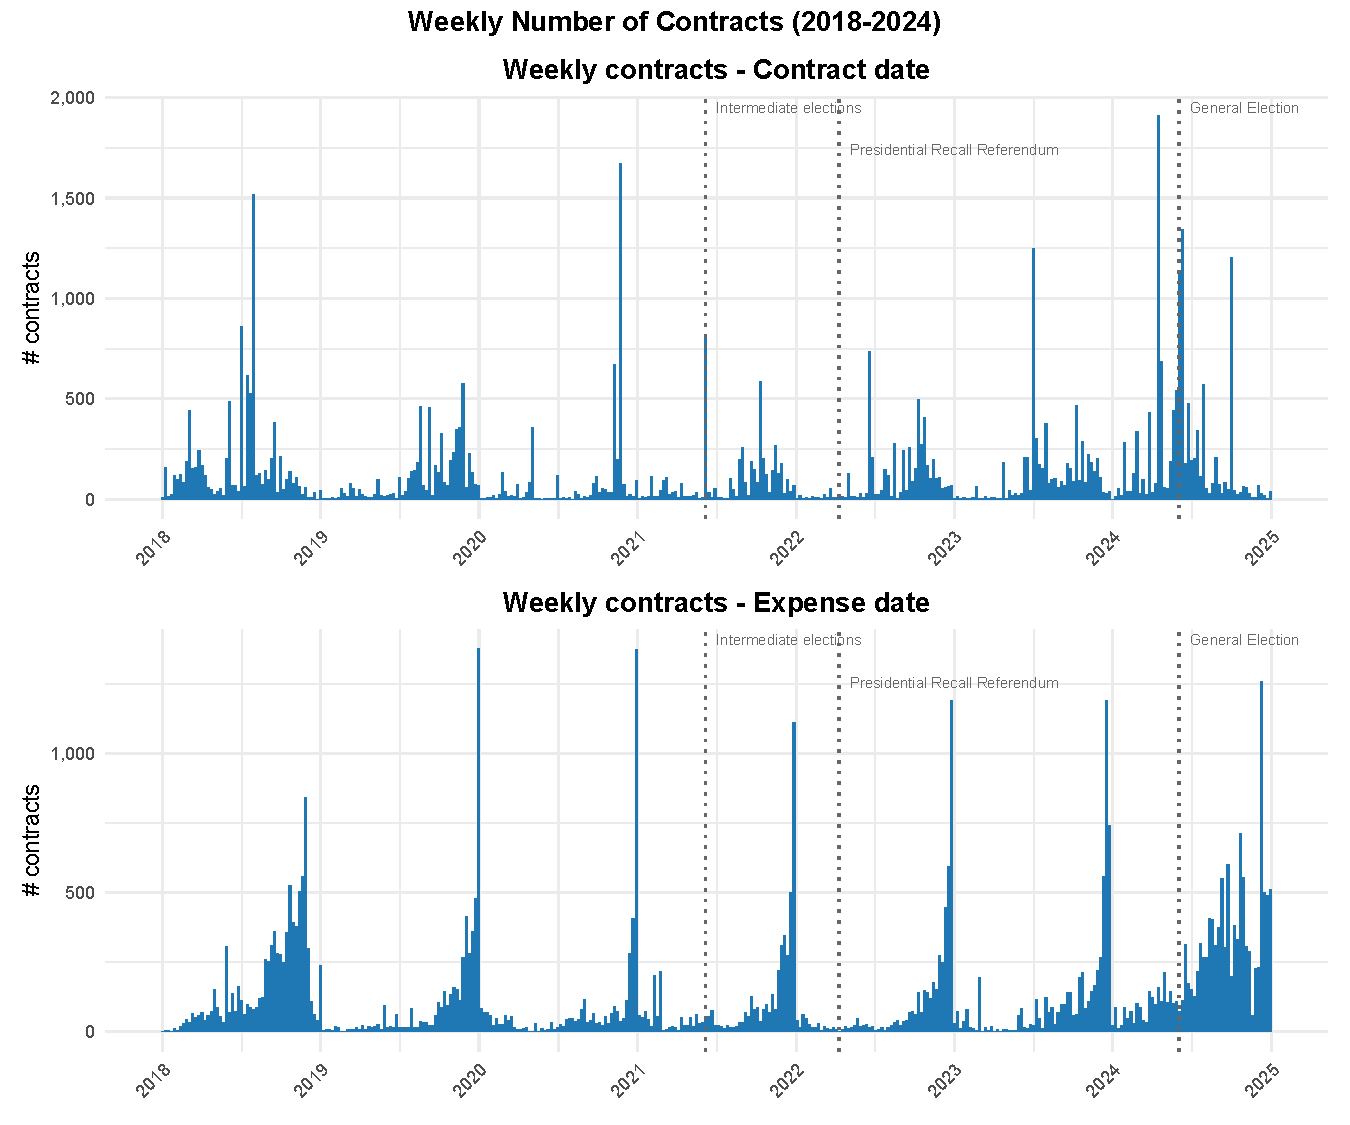
\includegraphics[width=\textwidth]{figures/descriptive_stats/01_count_weekly.pdf}
   \caption*{ \footnotesize{\textit{Note:} This figure presents the number of contracts assigned (top panel) and payed (lower panel) from 2018 to 2024 for the federal advertising spending from the Mexican government. Data was obtained from COMSOC}}
\end{figure}

First, this graph implicitly assumes that the federal government allocates contracts asynchronously across time. This may be true, or at least partly true, for the type of variation we want to capture: whether contracts are used to silence criticism or reward favorable coverage. However, contract timing may also vary significantly across the institutions that assign them. Figure \ref{fig:by_institution} addresses this possibility by plotting daily contracts by institution, showing that not all agencies follow the same allocation patterns.

This institutional variation is also substantively important. One could theorize why some institutions may be more likely than others to use advertising contracts to influence media behavior. For example, ISSSTE, the social security institution, shows much more timing variation than IMSS, the public health system. One possible explanation is that one institution may assign contracts for specific campaigns, such as vaccination campaigns, while the other may allocate contracts more regularly for general promotional purposes.

The figure also shows that the Tren Maya institution, associated with one of AMLO’s major infrastructure projects in southeastern Mexico, assigned a large number of contracts on a specific date. This is important because this date may have been announced in advance to media competitors, potentially affecting their behavior around the announcement.

Overall, these two figures suggest that there is meaningful time variation in contract allocation, but also important event-specific and campaign-specific variation. This variation can be exploited to better understand the process through which public advertising contracts are allocated. I discuss this further in the empirical strategy section.

\begin{figure}[htbp]
    \centering

    % Top row
    \begin{subfigure}[b]{\textwidth}
        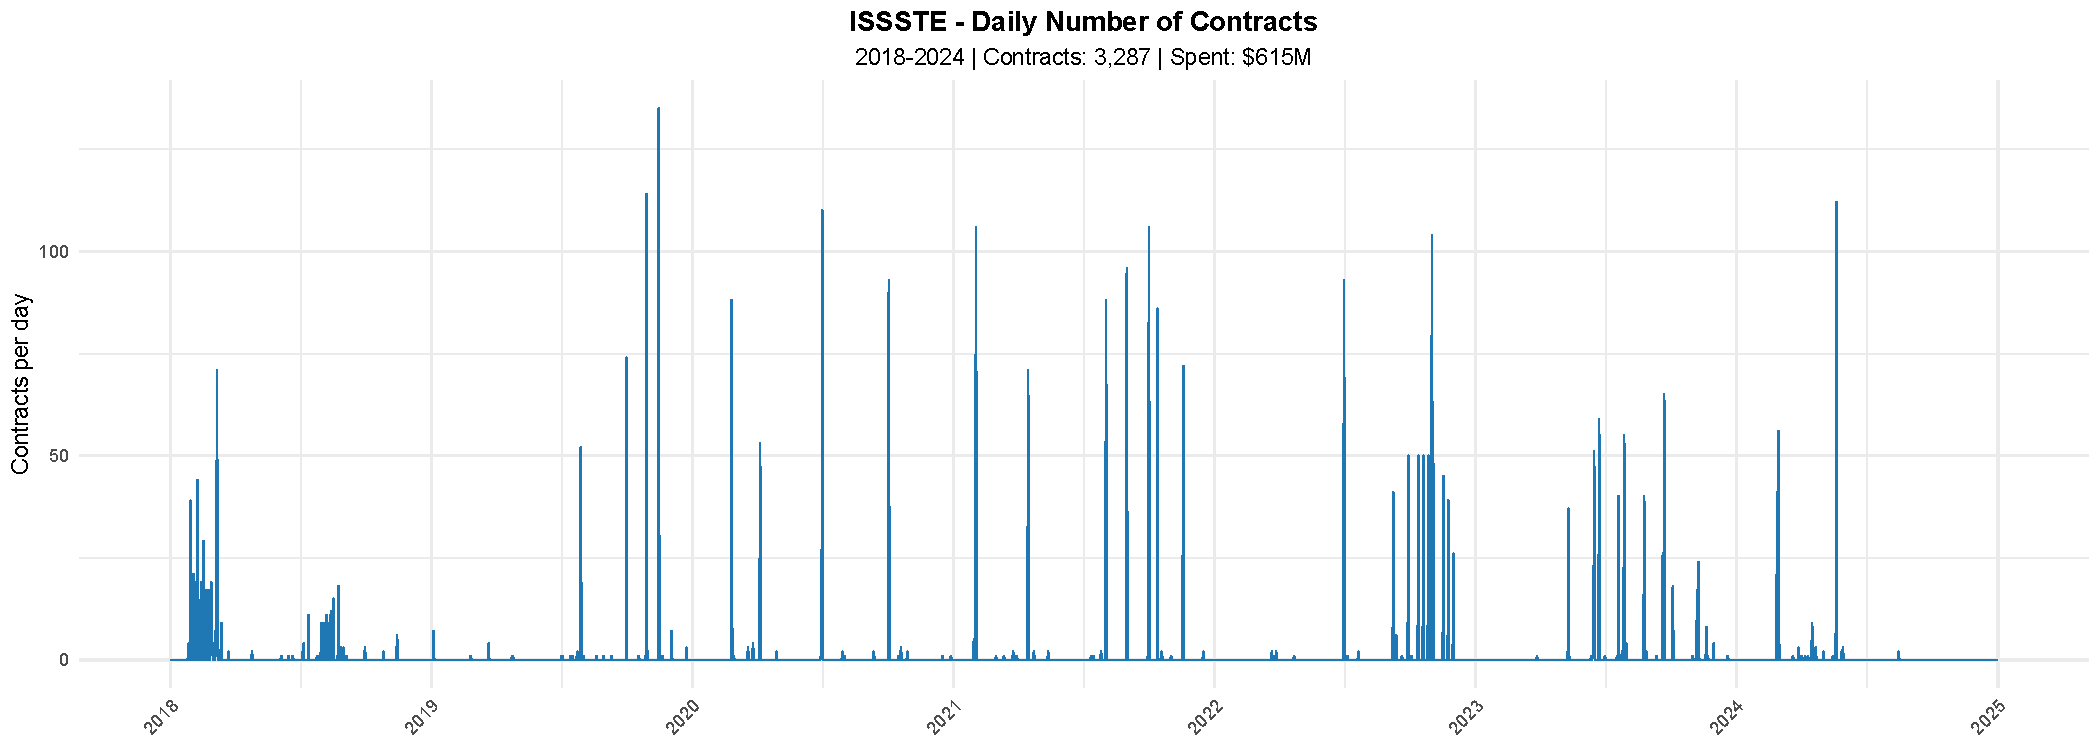
\includegraphics[width=\textwidth]{figures/descriptive_stats/top10_daily_contracts_04_issste.pdf}
        \caption{}
        \label{fig:ISSTE}
    \end{subfigure}
    \hfill
    \begin{subfigure}[b]{\textwidth}
        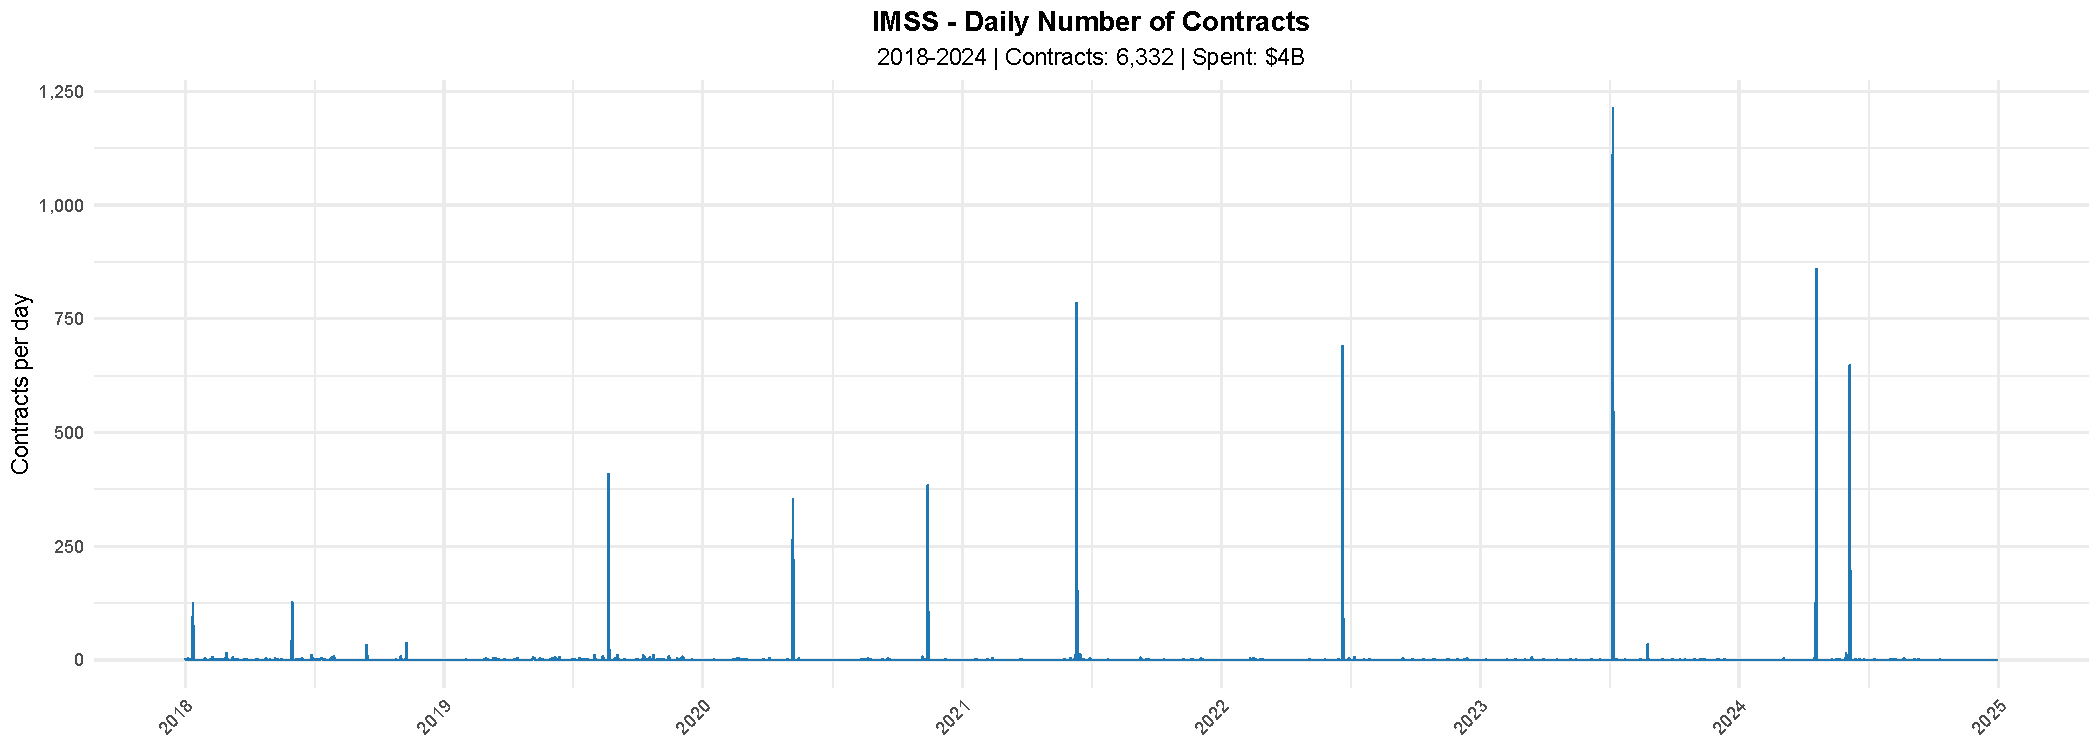
\includegraphics[width=\textwidth]{figures/descriptive_stats/top10_daily_contracts_01_imss.pdf}
        \caption{}
        \label{fig:imss}
    \end{subfigure}

    \vspace{0.5em}

    % Bottom row
    \begin{subfigure}[b]{\textwidth}
        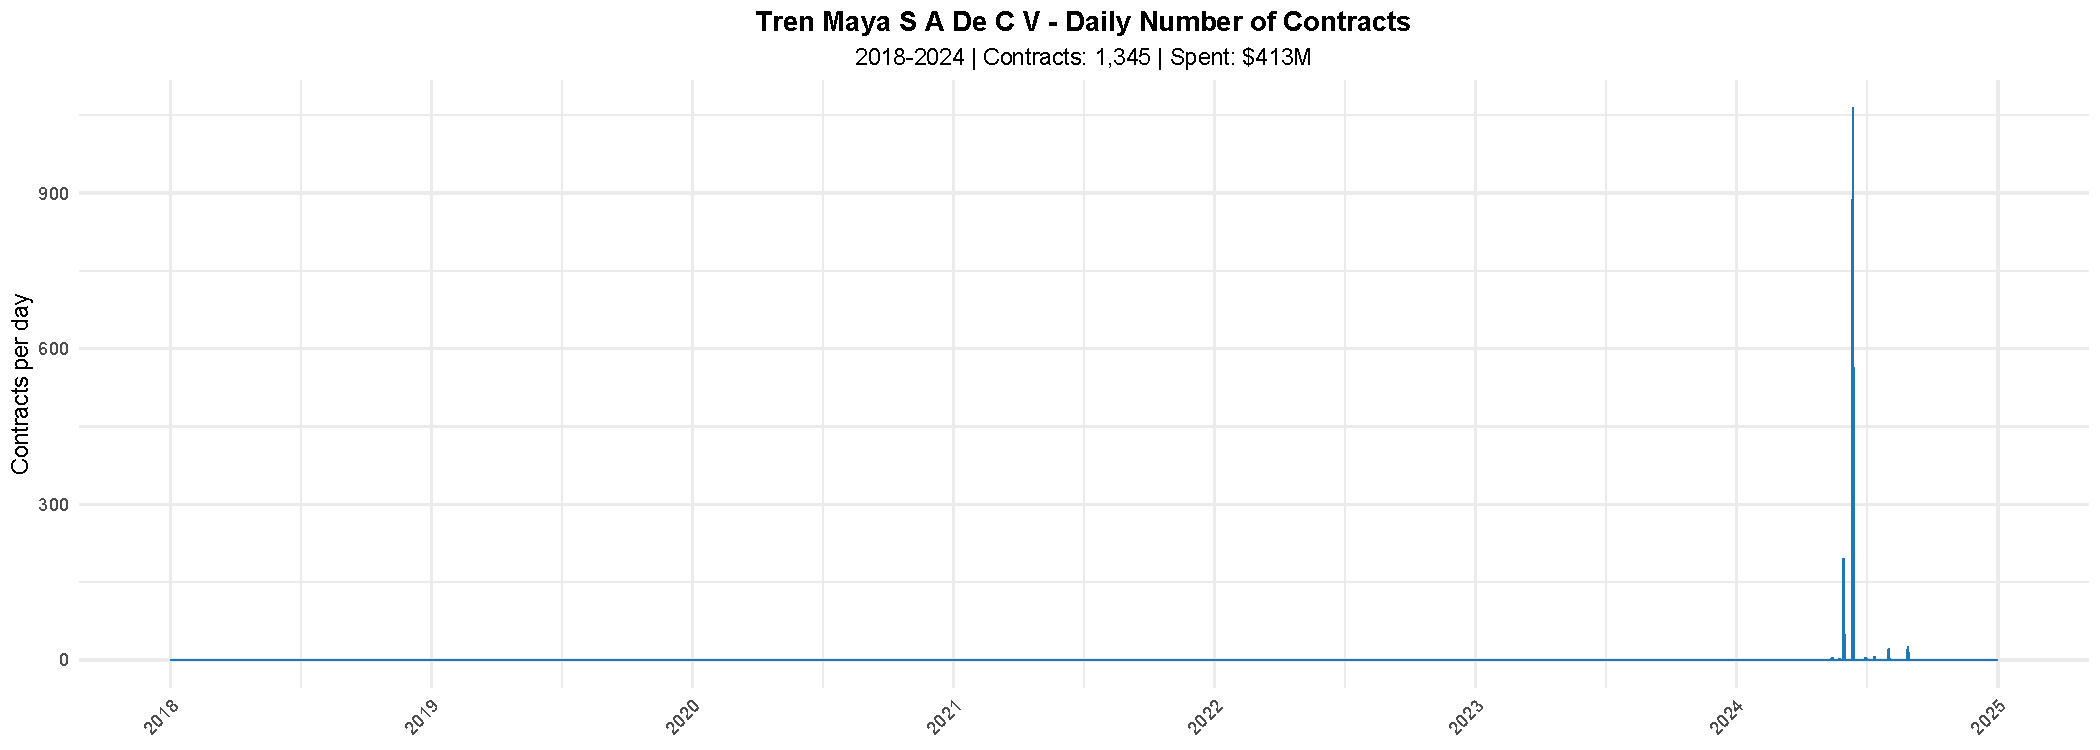
\includegraphics[width=\textwidth]{figures/descriptive_stats/top10_daily_contracts_07_tren_maya_s_a_de_c_v.pdf}
        \caption{}
        \label{fig:tren}
    \end{subfigure}
    \hfill


    \caption{Number of contracts by day for each institution.}
    \label{fig:by_institution}
\end{figure}


\subsection{Press conferences}

I have collected data on the official transcript of each morning press conference held by President López Obrador (a total of 1,423 conferences during his term). Additionally, I obtained through a Freedom of Information Request the media outlet of journalists attending each conference. This allows me to compile a comprehensive list of media outlets that have entered and participated in these press conferences. For initial analysis I have already extracted the information of journalists and media outlets that participated in the conference, using GPT and the structure of the conference.

\begin{figure}[!htpb]
   \centering
   \small
   \caption{}
   \label{fig:attendance_ov_time}
   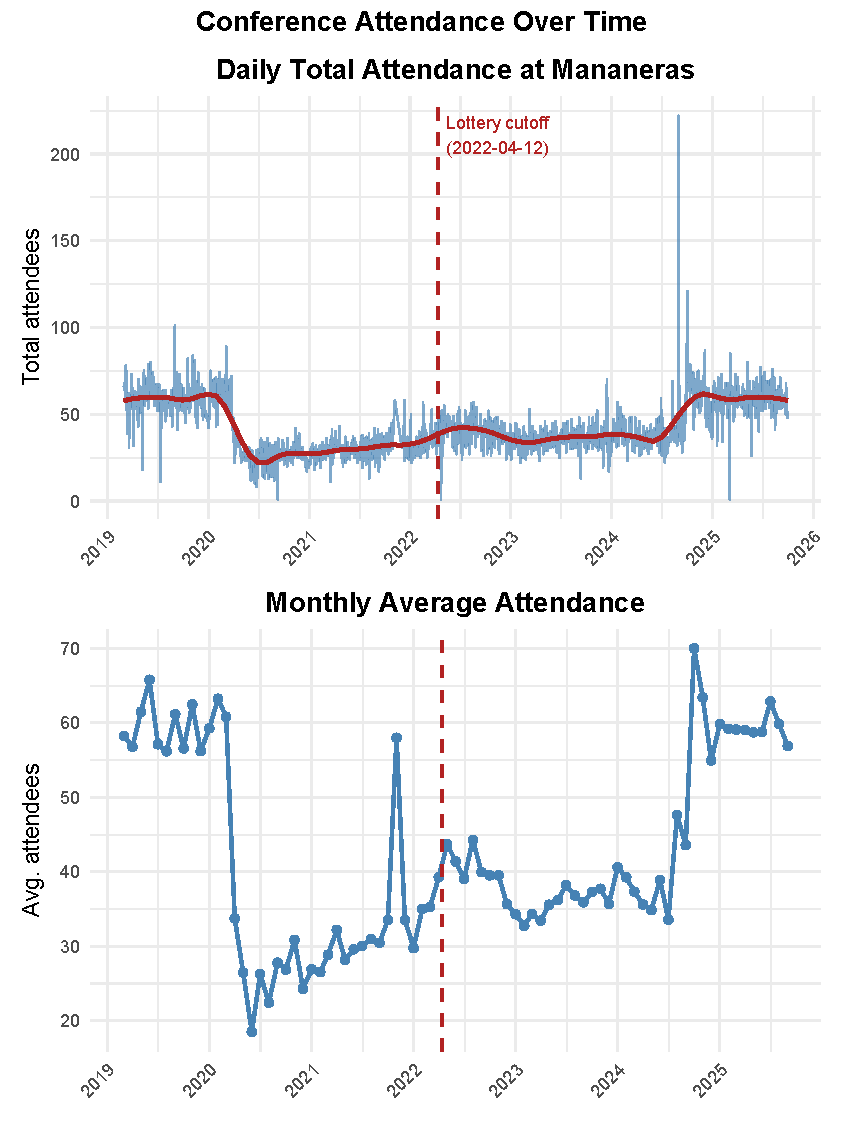
\includegraphics[width=\textwidth]{figures/descriptive_stats/01_conference_attendance_timeseries.pdf}
   \caption*{ \footnotesize{\textit{Note:} Conference Attendance over time}}
\end{figure}

A few patterns from Figure \ref{fig:attendance_ov_time}. First, attendance exhibits several clear structural shifts over time.
These are largely driven by institutional factors—such as changes in the venue’s overall capacity or the
relocation of conferences to other states—rather than by changes in demand to attend the press conferences
themselves. The large increase toward the end of the series corresponds to the beginning of President Claudia
Sheinbaum’s administration, when capacity expanded while the lottery system remained in place during the
first year.

More importantly for the design, the daily series suggests that there is no meaningful change in venue
capacity around the date when the lottery rule changed. In other words, the institutional change in the
allocation mechanism does not appear to coincide with a change in the number of available seats. This
implies that the shift in the assignment mechanism primarily affects who is able to ask a question, rather
than how many people can attend.

\begin{figure}[!htpb]
   \centering
   \small
   \caption{}
   \label{fig:att_top}
   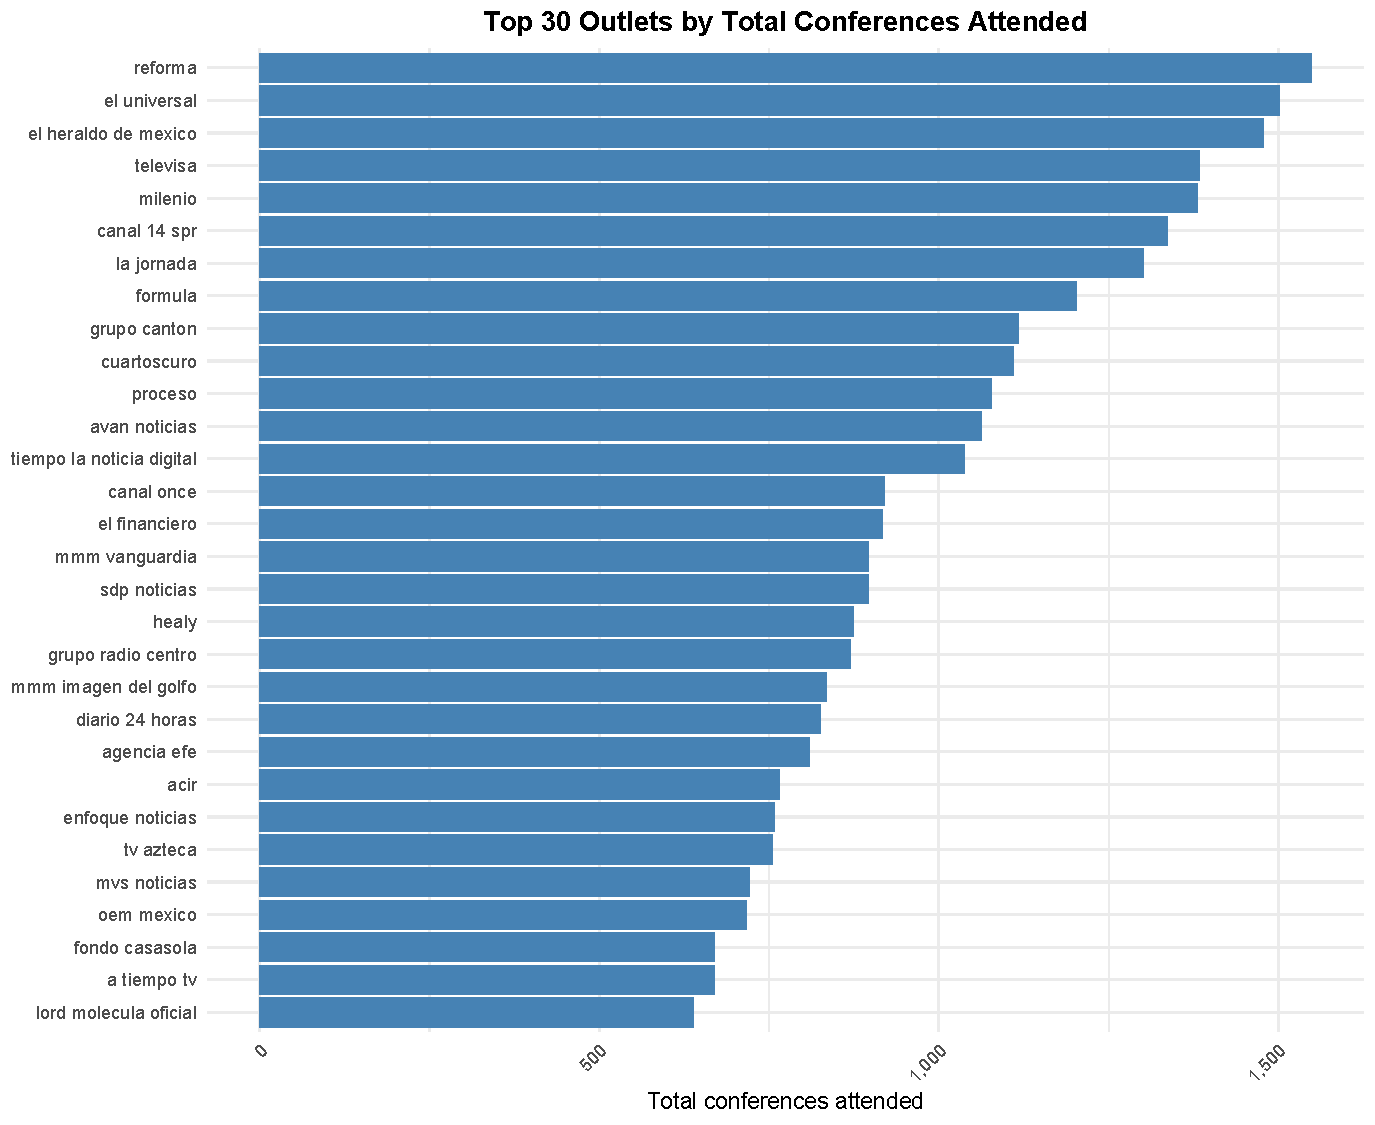
\includegraphics[width=\textwidth]{figures/descriptive_stats/02a_top30_outlets.pdf}
   \caption*{ \footnotesize{\textit{Note:} Attendance record by outlet}}
\end{figure}

Figure \ref{fig:att_top} shows that large outlets, regardless of ideology or political alignment, are those that attend the conference
most frequently. Reforma (oppositional, right-leaning), El Universal (oppositional), La Jornada (aligned,
left-leaning), and Grupo Cantón (aligned) are all among the outlets with the highest attendance. Part
of this pattern likely reflects resource differences. Attending the conference is costly—it requires assigning
reporters, paying salaries, and dedicating time that could otherwise be spent covering other events—so larger
organizations are better positioned to participate consistently.
Given this structure, the presence of a lottery and the ability to control for attendance make this setting
particularly useful empirically. Conditional on being present at the conference, the lottery introduces within
day exogenous variation in which outlet is selected to ask a question, which I will leverage in the analysis.


\subsection{Media Viewership}

As an initial proxy for audience demand for both the conference and individual media outlets, I collected video-level information from YouTube for the relevant study period. This includes videos posted by the YouTube channels of media outlets that attended the conference, as well as videos from the official channel that livestreamed the conference.

Figure~\ref{fig:youtube} presents descriptive statistics from these data. Panel A shows a clear increase over time in media outlets’ use of YouTube, reflected in both the number of videos posted and measures of audience engagement. Panel B shows that the sample includes an active and heterogeneous ecosystem of YouTube channels, with substantial variation in posting frequency, subscriber counts, and account creation dates before the study period. Together, these patterns suggest that YouTube provides a useful source of outlet-level variation in audience demand and online visibility.

\begin{figure}[htbp]
    \centering

    \begin{subfigure}[b]{\textwidth}
        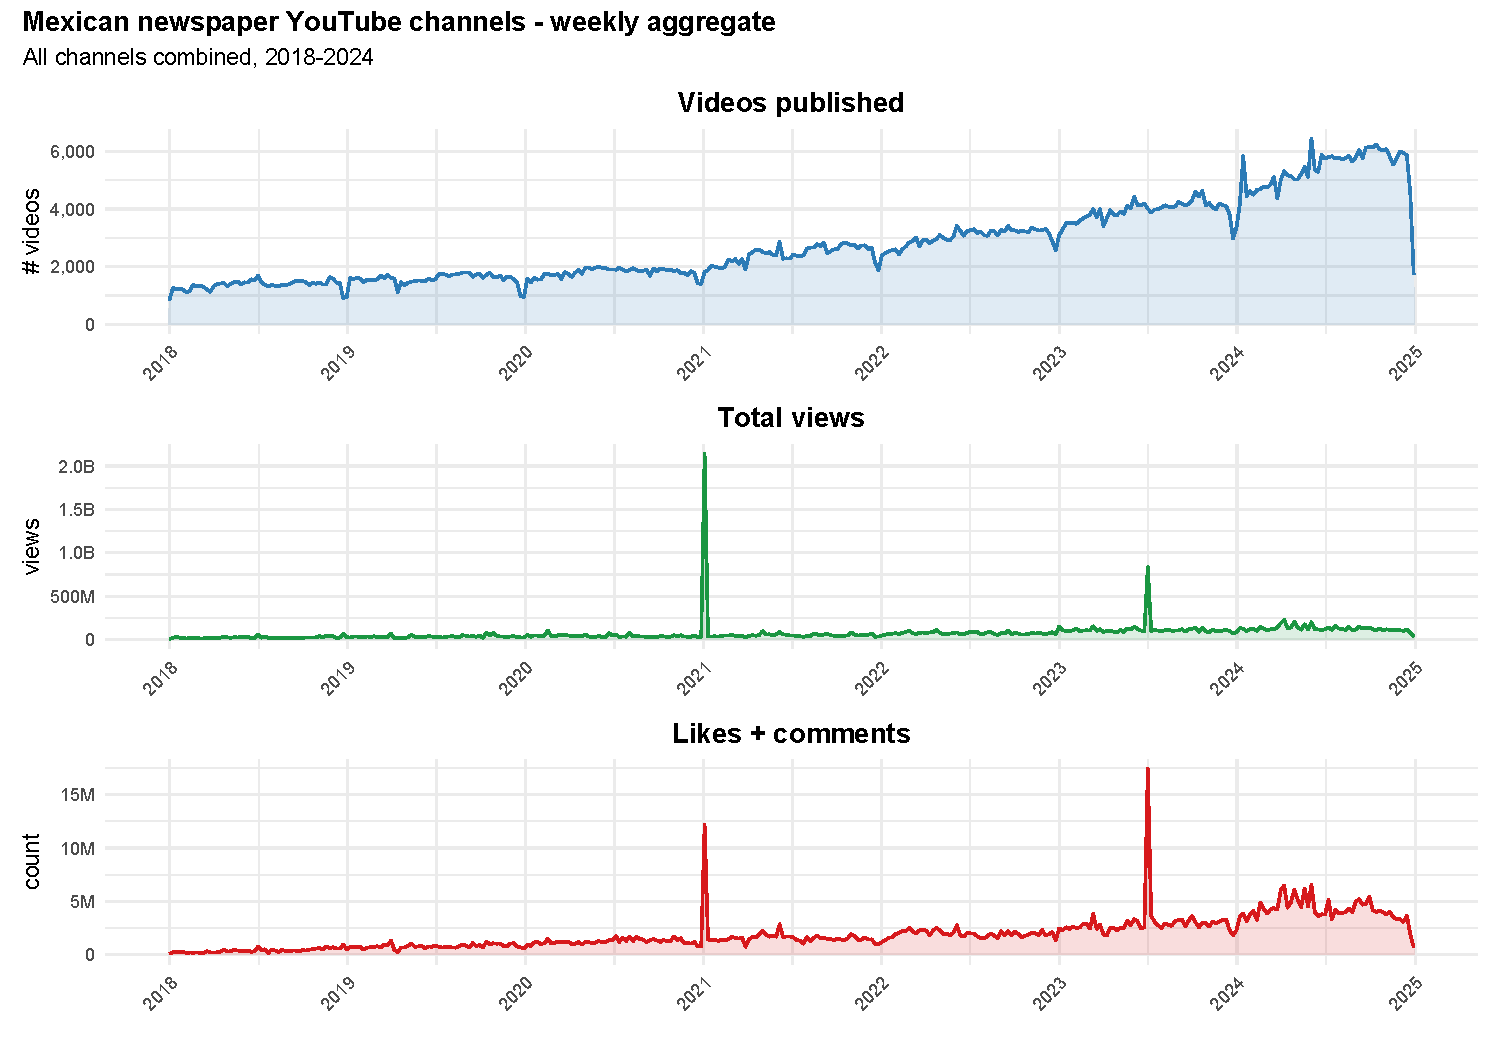
\includegraphics[width=\textwidth]{figures/descriptive_stats/fig1_timeseries_weekly.pdf}
        \caption{}
        \label{fig:imss}
    \end{subfigure}

    \vspace{0.5em}

    % Bottom row
    \begin{subfigure}[b]{\textwidth}
        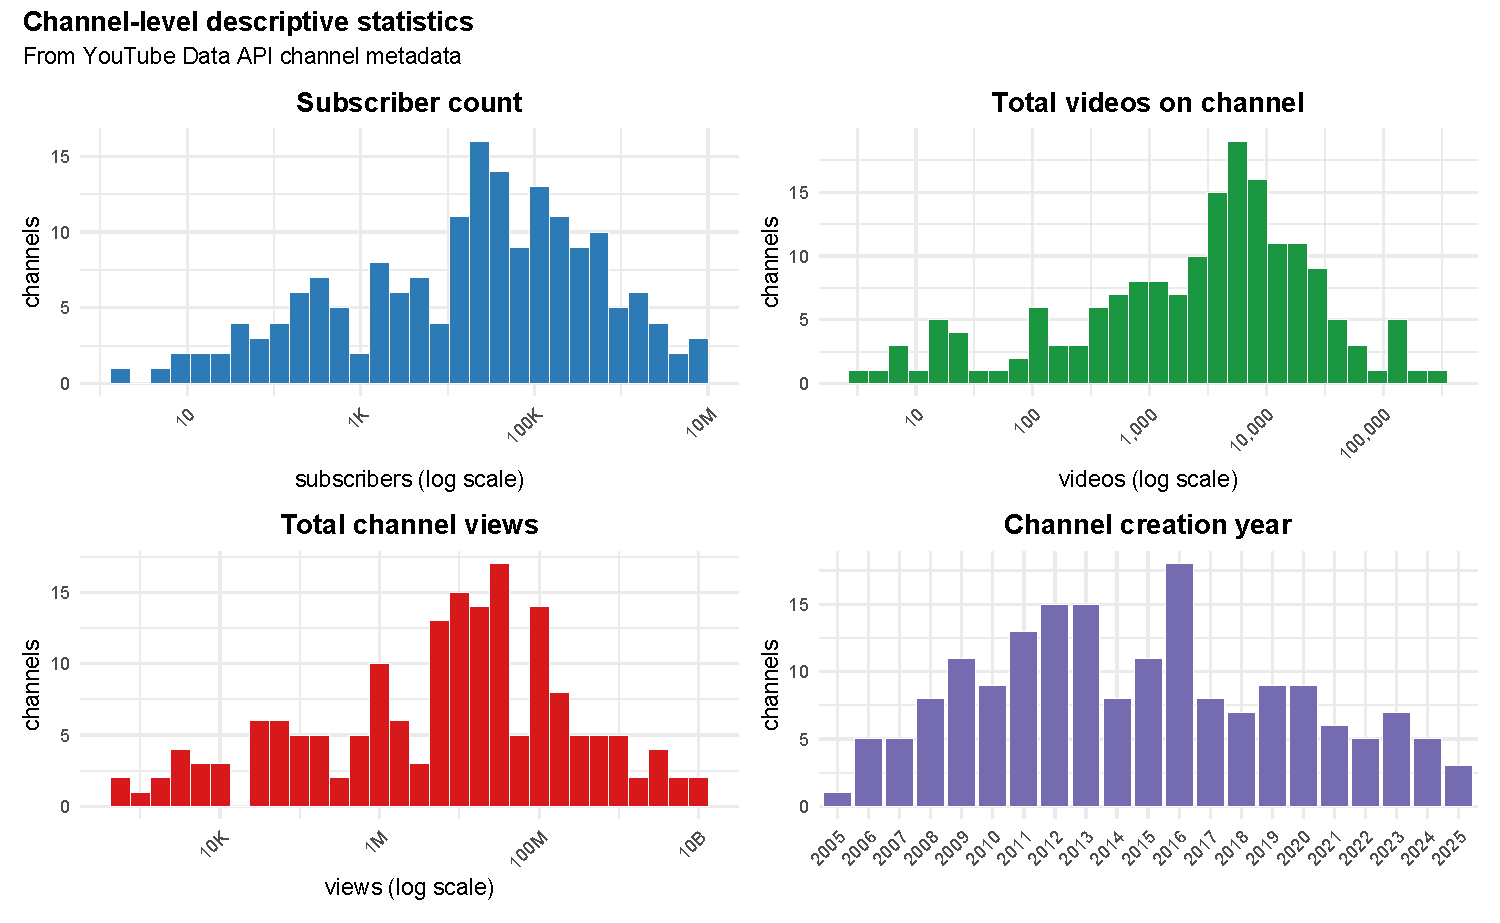
\includegraphics[width=\textwidth]{figures/descriptive_stats/fig2_channel_distributions.pdf}
        \caption{}
        \label{fig:tren}
    \end{subfigure}
    \hfill


    \caption{Youtube Channels Summary Stats by outlet}
    \label{fig:youtube}
\end{figure}

I have also started collecting Google Trends data to complement the YouTube measures of audience demand. I use two types of queries. First, I search for the names of media outlets to capture changes in public attention toward specific outlets over time. Second, I use the term mañanera to measure daily variation in broader public engagement with the morning conference itself. These data provide an additional measure of audience interest that is not limited to YouTube activity and can help capture changes in search behavior around specific conferences, questions, or political events.

In addition, I plan to complement these measures with Twitter data from the official handles of the media outlets. This would allow me to observe changes in posting behavior, engagement, and potentially the diffusion of conference-related content across platforms. Together, YouTube, Google Trends, and Twitter data would provide a broader picture of audience demand and media visibility, combining video consumption, search interest, and social media engagement.

\subsection{Other outcomes}

Other relevant outcomes include measures of public approval of the president. In particular, I use the daily AMLO tracking poll produced by Consulta Mitofsky and published at the weekly level, as shown in Figure~\ref{fig:tracking}. This measure is useful because it provides high-frequency variation in presidential approval during the period of the morning conferences. It can therefore help assess whether changes in the tone, composition, or visibility of the conference are associated with broader shifts in public support for the president.

\begin{figure}[!htpb]
   \centering
   \small
   \caption{}
   \label{fig:tracking}
   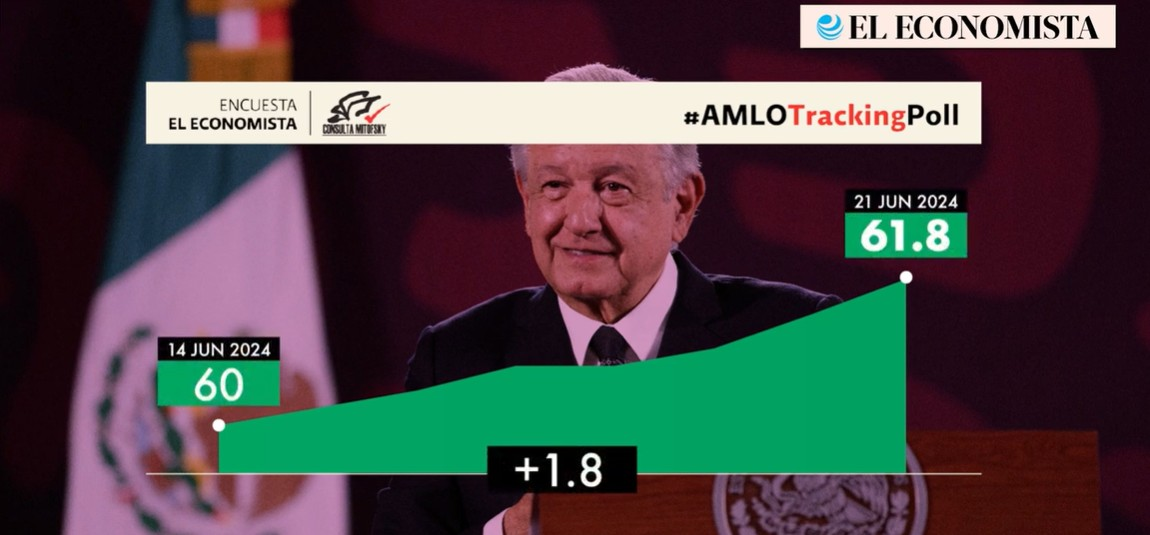
\includegraphics[width=\textwidth]{figures/descriptive_stats/amlotrackingpoll.jpg}
   \caption*{ \footnotesize{\textit{Note:} AMLOTrackingPoll Youtube Presentation}}
\end{figure}

